\section{Swing Prediction Model}

\subsection{Model Introduction}

In this section, we will primarily focus on establishing a model using the Gated Recurrent Unit (GRU) algorithm to 
predict momentum swings. We will break down the problems into three parts:

\begin{itemize}
    \item definition of the swing of the play
    \item data and label used to train GRU
    \item Gated Recurrent Unit (GRU) algorithm
\end{itemize}

\subsubsection{definition of the swing of the play}~{}

We first give the definition of the swings of the play.
Based on our previous definition of ``momentum,'' the significant changes of the game 
largely depend on the ``momentum'' of the two players. Therefore, we choose ``momentum'' to represent 
the swings of the play. The specific definition is as follows:\\

We use $\Delta f(t)$ to represent the difference in ``momentum'' between the two players., 
so it can be easily seen that if $\Delta f(t)$ and $\Delta f(t+1)$
have different signs, it indicates a ``swing'' in the game's momentum. 
In this way, we can define four states of ``momentum'' at time $t$:

$$states=\begin{cases}
    state1, &\text{if } \Delta f(t)>0 \text{ and } \Delta f(t+1)>0, \text{ which means stay positive}\\
    state2, &\text{if } \Delta f(t)<0 \text{ and } \Delta f(t+1)>0, \text{ which means rise from negative to positive}\\
    state3, &\text{if } \Delta f(t)<0 \text{ and } \Delta f(t+1)<0, \text{ which means stay negative}\\
    state4, &\text{if } \Delta f(t)>0 \text{ and } \Delta f(t+1)<0, \text{ which means decrease from positive to negative}
\end{cases}$$
Obviously, if state 2 or state 4 appears, we can determine that a swing has occurred. 

\subsubsection{Data and Label used to train GRU}~{}



\subsubsection{Use of Gated Recurrent Unit (GRU) Network}~{}

Gated Recurrent Units (GRUs) are a type of recurrent neural network (RNN) 
architecture that has gained popularity for sequential data processing. 
And it is appropriate for our many(10)-to-many(5) prediction model.

We will focus on a single unit of recurrent neural network to interpret the hidden mathematical principles:
\begin{figure}[H]
    \centering
    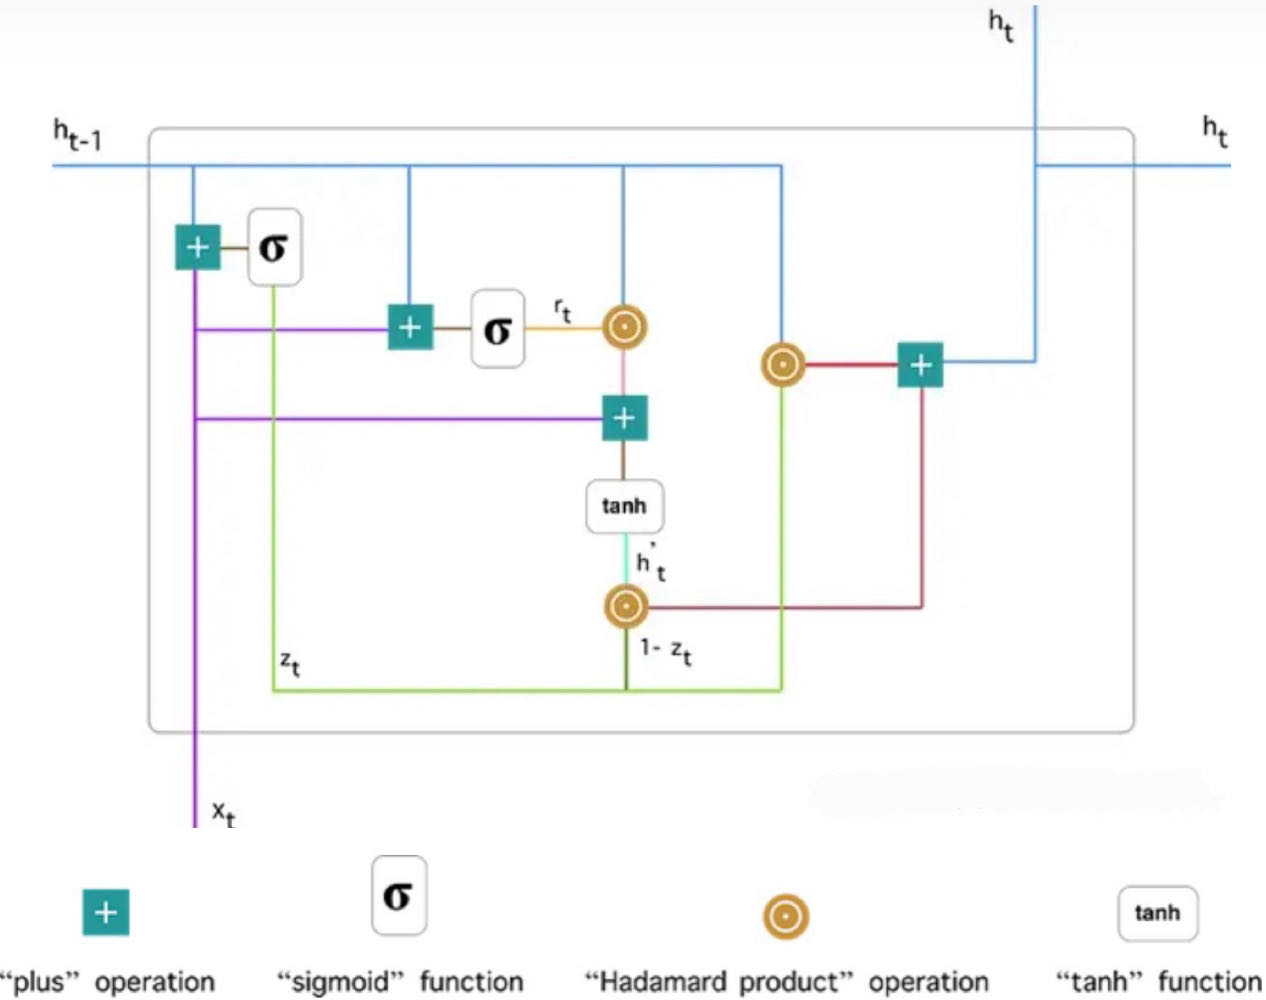
\includegraphics[scale=0.15]{mainmatter/imgs/6.jpg}
    \caption{Structure of GRU}
\end{figure}

\begin{enumerate}
    \item 
    The update gate at time step $t$ is computed using the following formula:  
    $$  z_t = \sigma(W_z \cdot x_t + U_z \cdot h_{t-1})  $$  
    Here, when $x_t$ is input to the network unit, 
    it is multiplied by its own weight $W_z$. 
    Similarly, $h_{t-1}$, which holds the information from the previous $t-1$ units, 
    is multiplied by its own weight $U_z$. These two results are then summed together 
    and passed through a sigmoid activation function to compress the result between 0 and 1. 
  
    \item 
    The essence of the reset gate is for the model to decide how much past information to forget. To compute it, we use:  
    $$  r_t = \sigma(W_r \cdot x_t + U_r \cdot h_{t-1})  $$  

    \item 
    The computation of the new memory content using the reset gate is as follows:  
    $$ h_t'= tanh(Wx_t+r_t\odot Uh_{t-1})$$

    \item 
    The computation for the new memory content $h_t$ using the update gate is as follows:  
    $$ h_t=z_t\odot h_{t-1}+(1-z_t)\odot h_t'$$ 
\end{enumerate}



\subsection{Visualization and Analysis}

calculate the match percentage of each match between the prediction model and the result from AHP.

\subsection{Weight of Factors}

Permutation Feature Importance theory is used to measure the importance of a feature by calculating 
the increase in the model's prediction error after permuting the feature.

\subsubsection{Permutation Feature Importance theory}~{}

We measure the importance of a feature by calculating the increase in the model’s prediction error 
after permuting the feature. A feature is “important” if shuffling its values increases the model error, 
because in this case the model relied on the feature for the prediction. A feature is “unimportant” if 
shuffling its values leaves the model error unchanged, because in this case the model ignored the feature 
for the prediction. 

\begin{algorithm}  
    \caption{Permutation Feature Importance}  
    \textbf{Input:} Trained model $\hat{f}$, feature matrix $X$, target vector $y$, error measure $L(y, \hat{f})$.  
      
    Estimate the original model error $e_{orig} = L(y, \hat{f}(X))$ (e.g. mean squared error)  
      
    \textbf{For} each feature $j \in \{1, ..., p\}$ \textbf{do:}  
      
    \quad\quad $\circ$ Generate feature matrix $X_{perm}$ by permuting feature $j$ in the data $X$. This breaks the association between feature $j$ and true outcome $y$.  
      
    \quad\quad $\circ$ Estimate error $e_{perm} = L(Y, \hat{f}(X_{perm}))$ based on the predictions of the permuted data.  
      
    \quad\quad $\circ$ Calculate permutation feature importance as quotient $FI_j = e_{perm} / e_{orig}$ or difference $FI_j = e_{perm} - e_{orig}$  
      
    Sort features by descending FI.
\end{algorithm}

If using match data of multiple different players, the factor with bigger weight is effective to 
all players.

\subsection{Advice against Opponent Based on Weight of Factors}

If using match data of a single player, the factor with bigger weight is extremely effective to 
this player.

Now we have finished Problem 3.

\subsection{Prediction Error compared with AHP model outcome}

Overlap rate of the prediction model and the result from AHP is?

\paragraph{Factors we may fail to consider}

First of all, the AHP model is not considering all possible factors to momentum.
For example, the.
So the overlap rate's effectiveness is limited.

Then, from the conclusion of problem 2, momentum only has one order of autocorrelation.
So when we try to predict the far future momentum, there's no reason to be accurate.